\documentclass[class=article,10pt,crop=false]{standalone}
\usepackage{standalone}
\usepackage{preamble}

\begin{document}
\begin{multicols}{2}[\section{Linear geometry}]
\subsection{The foundations of geometry}
In this section we will only study geometry in the plane.
\subsubsection*{Euclidean geometry}
\begin{axiom}[Euclid's axioms]
\hfill
\begin{enumerate}
    \item It is possible to draw, from any point to any point, a straight line.
    \item It is possible to extend any segment by either of its two ends. 
    \item With center at any point it is possible to draw a circle that passes through any other point. 
    \item All right angles are equal.
    \item If a line segment intersects two straight lines forming two interior angles on the same side that sum to less than two right angles, then the two lines, if extended indefinitely, meet on the side on which the angles sum to less than two right angles.
    \item[5$'$.] \textit{(Playfair's axiom)} Given a line and a point not on it, at most one line parallel to the given line can be drawn through the point.
\end{enumerate}
\end{axiom}
\subsubsection*{Hilbert's axioms}
\begin{definition}
In elementary plane geometry\footnote{In this section we only study the geometry in the plane.}, there are two types of objects, \textit{points} and \textit{lines}, which can have three types of relationships between them:
\begin{itemize}
    \item An \textit{incidence relation}. We say, for example, that a point lies on a line or a line passes through a point.
    \item An \textit{order relation}. We say, for example, that a point lies between two other points.
    \item A \textit{congruence relation}. We say, for example, that a segment is congruent to another or an angle is congruent to another\footnote{We will use the notation $\equiv$ to say that two angles or segments are congruent.}.
\end{itemize}
\end{definition}
\begin{axiom}[Incidence axioms]
\label{1}
\hfill
\begin{enumerate}
    \item For every two points there exists no more than one line containing both.
    \item There exist at least two points on a line.
    \item There exist at least three points that do not lie on the same line.
\end{enumerate}
\end{axiom}
\begin{axiom}[Order axioms]
\label{2}
\hfill
\begin{enumerate}
    \item If a point $B$ lies between $A$ and $C$, then $B$ lies between $C$ and $A$ and there exists a line containing the distinct points $A,B,C$.
    \item If $A$ and $B$ are two points, there exists at least one point $C$ such that $B$ lies between $A$ and $C$.
    \item Given three point on a line, there is no more than one which lies between the other two.
    \item \textit{(Pasch's axiom)} Let $A,B,C$ be three points not-lying in the same line and let $r$ be a line not passing through any of the points $A,B,C$ and passing through a point of the segment $AB$. Then it also passes through either a point of the segment $BC$ or a point of the segment $AC$.
\end{enumerate}
\end{axiom}
\begin{definition}
A \textit{ray} or \textit{half-line} is a point $A$, called vertex, and all the points of a line passing through $A$ lying on the same side with respect to $A$.
\end{definition}
\begin{definition}
A \textit{half-plane} is a straight line $r$ and all the points lying on the same side with respect to $r$.
\end{definition}
\begin{definition}
An \textit{angle} is a non-ordered pair of rays with same vertices that belong to different straight lines.
\end{definition}
\begin{axiom}[Congruence axioms]
\label{3}
\hfill
\begin{enumerate}
    \item Congruence of angles and congruence of rays are equivalence relations.
    \item Let $a$ and $b$ be two lines not necessarily different, $A$ and $B$ be points on $a$ and $A'$ be a point on $b$. We fix a side of the line $b$ with respect to $A'$. Then, there exists a point $B'$ lying on this side of $b$ such that $AB\equiv A'B'$.
    \item Let $a,a'$ be two lines not necessarily different. Let $AB,BC$ be segments on $a$ that intersect only in one point and $A'B',B'C'$ be segments on $a'$ that also intersect only in one point. If $AB\equiv A'B'$ and $BC\equiv B'C'$, then $AC\equiv A'C'$.
    \item Let $\angle hk$ be an angle, $k'$ be a ray and $H$ be one of the two half-planes that $k'$ defines. Then, there is one and only one angle $\angle h'k'$ such that $\angle hk\equiv\angle h'k'$ and $h'$ belongs to $H$.
    \item \textit{(SAS criterion)} Consider two triangles\footnote{We will use the following notation with respect to the angles of a triangle $ABC$: $\alpha=\angle CAB$, $\beta=\angle ABC$ and $\gamma=\angle BCA$.} $ABC$ and $A'B'C'$ (not necessarily different). If $AC\equiv A'C'$, $AB\equiv A'B'$ and $\alpha\equiv\alpha'$, then $\beta\equiv\beta'$.
\end{enumerate}
\end{axiom}
\begin{axiom}[Continuity axioms]
\label{4}
\hfill
\begin{enumerate}
    \item \textit{(Axiom of Archimedes)} If $AB$ and $CD$ are any segments, then there exists a number $n$ such that $n$ segments $CD$ constructed contiguously from $A$, along the ray from $A$ to $B$, will pass beyond the point $B$.
    \item \textit{(Axiom of completeness)} An extension of a set of points on a line with order and congruence relations that would preserve the relations existing among the original elements as well as the rest of the axioms is impossible.
    \item \textit{(RC)} If a straight line passes through a point inside a circle, it intersects the circle in two points.
    \item \textit{(CC)} If a circle passes through points inside and outside another circle, the two circle intersect in two points.
\end{enumerate}
\end{axiom}
\begin{axiom}[Axiom of Parallels]
\label{5}
Let $a$ be any line and $A$ be a point not on it. Then there is at most one line that passes through $A$ and does not intersect $a$.
\end{axiom}
\begin{definition}
Different types of geometry: 
\begin{itemize}
    \item A \textit{Hilbert plane} is a geometry where axioms \ref{1}, \ref{2} and \ref{3} are satisfied.
    \item A \textit{Pythagorean plane} is a Hilbert plane in which axiom of Parallels is satisfied.
    \item An \textit{Euclidean plane} is a Pythagorean plane in which axioms RC and CC are satisfied.
    \item The \textit{Cartesian geometry of $\mathbb{R}^2$} is the unique geometry satisfying all Hilbert's axioms.
\end{itemize}
\end{definition}
\subsubsection*{Absolute geometry}
\begin{definition}
\textit{Absolute geometry} is the part of Euclidean geometry that only uses axioms \ref{1}, \ref{2} and \ref{3}.
\end{definition}
\begin{theorem}
In an isosceles triangles, the angles opposite the congruent sides are congruent.
\end{theorem}
\begin{theorem}[SAS criterion]
If two sides of a triangle and the angle between them are congruent to the corresponding sides and angle of a second triangle, then the two triangles are congruent.
\end{theorem}
\begin{theorem}
Adjacent angles of congruent angles are congruent.
\end{theorem}
\begin{theorem}
Opposite angles\footnote{Opposite angles are angles that are opposite each other when two lines intersect.} are congruent.
\end{theorem}
\begin{theorem}
If $A$ and $B$ are each on one of the sides of an angle with vertex $O$, any ray with vertex $O$ that passes through an interior point of the angle intersects the segment $AB$.
\end{theorem}
\begin{theorem}
There exist right angles.
\end{theorem}
\begin{theorem}
Let $\alpha,\alpha',\beta,\beta'$ be angles. If $\alpha\equiv\alpha'$ and $\beta\equiv\beta'$, then $\alpha+\beta\equiv\alpha'+\beta'$.
\end{theorem}
\begin{theorem}[SSS criterion]
If two triangles have all its sides congruent, they have all its angles congruent.
\end{theorem}
\begin{theorem}
Right angles are congruent.
\end{theorem}
\begin{theorem}[Exterior angle theorem]
An exterior angle of a triangle is greater than any of the non-adjacent interior angles.
\end{theorem}
\begin{theorem}
If $\ell$ is a line and $P$ is a point not lying on $\ell$, there exists a line $L$ passing through $P$ and such that not intersects $\ell$.
\end{theorem}
\begin{theorem}[ASA criterion]
If two triangles have a side and the two angles of this side congruent, the triangles are congruent.
\end{theorem}
\begin{theorem}[SAA criterion]
If two triangles have a side, an angle of this side and the angle opposite to this side congruent, the triangles are congruent.
\end{theorem}
\begin{theorem}
In any triangle the greater side is opposite to the greater angle.
\end{theorem}
\begin{theorem}
If a triangle has two congruent angles, it is isosceles.
\end{theorem}
\begin{theorem}
Every segment has a midpoint.
\end{theorem}
\begin{theorem}
Every angle has an angle bisector.
\end{theorem}
\begin{theorem}
Every segment has a perpendicular bisector.
\end{theorem}
\begin{theorem}[Saccheri–Legendre theorem]
The sum of the angles of a triangle is at most two right angles.
\end{theorem}
\subsubsection*{Cartesian geometry}
\begin{definition}
An \textit{ordered field $k$} is a field together with a total order of its elements, satisfying:
\begin{itemize}
    \item $x\leq y\implies x+z\leq y+z$ $\forall z\in k$.
    \item $x,y\geq 0\implies xy\geq 0$.
\end{itemize}
\end{definition}
\begin{definition}
We say a field $k$ is \textit{Pythagorean} if $\forall a\in k$, $1+a^2=b^2$ for some $b\in k$.
\end{definition}
\begin{theorem}
$k^2$ is a Pythagorean plane if and only if $k$ is an ordered Pythagorean field.
\end{theorem}
\begin{definition}
An ordered field $k$ is \textit{Archimedean} if axiom of Archimedes is valid in $k$.
\end{definition}
\begin{definition}
An ordered field $k$ is \textit{Euclidean} if $\forall a\in k$, $a>0$, there exists a $b\in k$ such that $b^2=a$.
\end{definition}
\begin{theorem}
$k^2$ is a Euclidean plane if and only if $k$ is an ordered Euclidean field.
\end{theorem}
\begin{definition}
The smallest Pythagorean field is called \textit{Hilbert field} ($\Omega$) and it can be defined as the intersection of all Pythagorean fields of $\mathbb{R}$. Alternatively, it can be defined as the field whose elements are the real numbers obtained from rational numbers with the operations of addition, subtraction, multiplication, multiplicative inverse and the operation $a\mapsto\sqrt{1+a^2}$.
\end{definition}
\begin{definition}
The smallest Euclidean field is called \textit{constructible field} ($\mathbb{K}$) and it can be defined as the intersection of all Euclidean fields of $\mathbb{R}$. Alternatively, it can be defined as the field whose elements are the real numbers obtained from rational numbers with the operations of addition, subtraction, multiplication, multiplicative inverse and the square root of positive numbers.
\end{definition}
\subsubsection*{Non-Euclidean geometries}
\begin{definition}[Hyperbolic geometry]
\textit{Hyperbolic geometry} is the non-Euclidean geometry where axiom of Parallels fails.
\end{definition}
\begin{prop}
Properties of hyperbolic geometry:
\begin{itemize}
    \item There are infinity lines parallel to a given line $\ell$ that pass through a point not lying on $\ell$.
    \item There are lines inside an angle that do not intersect the sides of the angle.
    \item The sum of the angles of any triangle is less than two right angles.
\end{itemize}
\end{prop}
\begin{definition}
Hyperbolic geometry models:
\begin{itemize}
    \item Beltrami-Klein model:
    \begin{itemize}
        \item Points: $\mathcal{K}:=\{(x,y)\in\mathbb{R}^2:x^2+y^2<1\}$.
        \item Lines: Lines of $\mathbb{R}^2$ that intersect with $\mathcal{K}$.
        \item Incidence and order relations are the same as in ordinary Euclidean geometry of $\mathbb{R}^2$.
        \item Two segments $AB,A'B'\in\mathcal{K}$ are congruent if and only if there is an Euclidean motion\footnote{See section \ref{LG-euclidean_motion}.} $f$ such that $f(A)=A'$ and $f(B)=B'$. Two angles $hk,h'k'\in\mathcal{K}$ are congruent if and only if there is an Euclidean motion $f$ such that $f(h)=h'$ and $f(k)=k'$.
    \end{itemize}
    \begin{minipage}{\linewidth} 
        \centering
        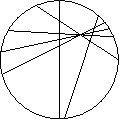
\includegraphics[width=0.6\linewidth]{Mathematics/2nd/Linear_geometry/Images/klein.tex} 
        \captionof{figure}{Beltrami–Klein model.}
    \end{minipage} 
    \item Poincaré disk model:
    \begin{itemize}
        \item Points: $\mathcal{D}:=\{(x,y)\in\mathbb{R}^2:x^2+y^2<1\}$.
        \item Lines: 
        \begin{enumerate}
            \item Lines of $\mathbb{R}^2$ that pass through the origin.
            \item Circles of $\mathbb{R}^2$ that intersect orthogonally the circle $\mathcal{C}=\{(x,y)\in\mathbb{R}^2:x^2+y^2=1\}$.
        \end{enumerate}
        \item Incidence and order relations are the same as in ordinary Euclidean geometry of $\mathbb{R}^2$.
        \item Is a conformal model: The hyperbolic measure of an angle coincides with the Euclidean measure of it whereas the distance between two points $A,B\in\mathcal{D}$ is measured using the following formula: $$d_h(A,B):=-\log\frac{d(A,P)d(B,Q)}{d(A,Q)d(B,P)}.$$ where $P,Q\in\mathcal{C}$ are the boundary points of $\mathcal{D}$ on the line passing through $A$ and $B$ so that $A$ lies between $P$ and $B$.
    \end{itemize}
    \begin{minipage}{\linewidth} 
        \centering
        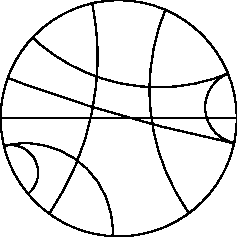
\includegraphics[width=0.6\linewidth]{Mathematics/2nd/Linear_geometry/Images/disk.tex} 
        \captionof{figure}{Poincare disk model.}
    \end{minipage} 
    \item Poincaré half-plane model:
    \begin{itemize}
        \item Points: $\mathcal{H}:=\{(x,y)\in\mathbb{R}^2:y>0\}$.
        \item Lines:
        \begin{enumerate}
            \item Vertical straight lines of $\mathbb{R}^2$.
            \item Circles of $\mathbb{R}^2$ with center on the $x$-axis.
        \end{enumerate}
        \item Incidence and order relations are the same as in ordinary Euclidean geometry of $\mathbb{R}^2$.
        \item Is a conformal model. The distance between two points $A,B\in\mathcal{D}$ is measured using the following formula: $$d_h(A,B):=-\log\frac{d(A,P)d(B,Q)}{d(A,Q)d(B,P)}.$$ where $P,Q\in\{(x,y)\in\mathbb{R}^2:y=0\}$ are the points where the semicircle meet the boundary line $y=0$.
    \end{itemize}
    \begin{minipage}{\linewidth} 
        \centering
        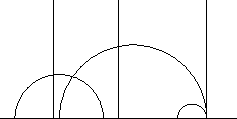
\includegraphics[width=0.6\linewidth]{Mathematics/2nd/Linear_geometry/Images/half.tex} 
        \captionof{figure}{Poincare half-plane model.}
    \end{minipage} 
\end{itemize}
\end{definition}
\begin{definition}[Non-Paschian geometry]
\textit{Non-Paschian geometry} is the non-Euclidean geometry where axiom of Archimedes fails.
\end{definition}
\begin{prop}[Construction of a non-Paschian geometry]
Suppose we have a total order relation $\unlhd$ on $\mathbb{R}$ such that:
\begin{enumerate}
    \item $x\unlhd y\implies x+z\unlhd y+z$ $\forall x,y,z\in\mathbb{R}$.
    \item $\exists a,b\in\mathbb{R}: a\unrhd 0, b\unrhd 1$ and $ab\unlhd 0$.
\end{enumerate}
Then, the ordinary affine geometry of $\mathbb{R}^2$ together with $\unlhd$, satisfy all Hilbert's axioms except Pasch's axiom.
\end{prop}
\begin{definition}[Non-SAS geometry]
\textit{Non-SAS geometry} is the non-Euclidean geometry where SAS criterion fails.
\end{definition}
\begin{prop}[Construction of a non-SAS geometry]
\hfill
\begin{itemize}
    \item Points: $\mathcal{S}=\{(x,y,z)\in\mathbb{R}^3:x+z=0\}=\{(x,y,-x)\in\mathbb{R}^3\}$.
    \item Lines: Ordinary straight lines of $\mathbb{R}^2$ contained in $\mathcal{S}$.
    \item Incidence and order relations are the same as in ordinary Euclidean geometry of $\mathbb{R}^2$.
    \item Congruence of angles is the same as in the ordinary geometry of $\mathbb{R}^3$. Congruence of segments is based in the following distance:  $$d'((x,y,-x),(x',y'-x'))^2=(x-x')^2+(y-y')^2.$$ That is, two segments are congruent if so are their projections to the plane $z=0$.
\end{itemize}
\end{prop}
\begin{definition}[Non-Archimedean geometry]
\textit{Non-Archimedean geometry} is the non-Euclidean geometry where SAS criterion fails.
\end{definition}
\subsubsection*{Axiomatic projective space}
\begin{definition}
An \textit{axiomatic projective space} is a system of points and lines with an incidence relation that satisfy:
\begin{enumerate}
    \item Every line contains at least 3 points
    \item Any two distinct points lie on a unique line.
    \item \textit{(Projective axiom)} If $A,B,C,D$ are four different points and lines $AB$ and $CD$ intersect, then lines $AC$ and $BD$ also intersect.
\end{enumerate}
\end{definition}
\begin{definition}
Let $X$ be a projective space. A \textit{projective subvariety of $X$} is a set $Z\ne\emptyset$ of points of $X$ such that if $x,y\in Z$ are different points, then all the points lying on the line passing through $x$ and $y$ belong to $Z$. Thus, $Z$ is also a projective space.
\end{definition}
\begin{prop}
Let $X$ be a projective space. The intersection of subvarieties of $X$ is also a subvariety of $X$.
\end{prop}
\begin{prop}
If $A$ and $B$ are subvarieties of a projective space $X$, we define its sum $A+B$ as the intersection of all subvarieties containing $A\cup B$. As a consequence, $A+B$ is a subvariety of $X$.
\end{prop}
\begin{definition}
Let $X,Y$ be a projective spaces. A \textit{collineation between $X$ and $Y$} is a bijection map $f:X\rightarrow Y$ such that $A,B,C\in X$ are three collinear points if and only if $f(A),f(B),f(C)\in Y$ are also collinear.
\end{definition}
\begin{definition}
If $X$ is a projective space, the \textit{dimension of $X$} is the maximum $n$ such that there is a chain of inclusions $$X_0\varsubsetneq X_1\varsubsetneq X_2 \varsubsetneq\cdots\varsubsetneq X_n,$$ where each $X_i$ is a non-empty subvariety of $X$. If this $n$ doesn't exist, we say $X$ has infinite dimension.
\end{definition}
\begin{definition}
\label{pproj}
A \textit{projective plane} is a projective space of dimension 2 that satisfies the following axioms:
\begin{enumerate}
    \item Any two distinct points lie on a unique line.
    \item Any two distinct lines meet on a unique point.
    \item There exist at least four points of which no three are collinear.
\end{enumerate}
\end{definition}
\begin{theorem}
$X$ is a projective space of dimension 2 if and only if $X$ satisfies axioms \ref{pproj}.
\end{theorem}
\begin{theorem}[Duality principle]
If a statement $\mathcal{P}$ (which only involves points and lines) is true in any projective plane, then the statement obtained from $\mathcal{P}$ exchanging points by lines (and correctly changing all the connectors to make a consistent statement) is also true in any projective plane.
\end{theorem}
\subsubsection*{Affine and projective spaces}
\begin{definition}
An \textit{affine plane} is a set of points and lines satisfying the following axioms:
\begin{enumerate}
    \item Any two distinct points lie on a unique line.
    \item If $r$ is a line and $P\notin r$ is a point, there exists a unique line $s$ such that $P\in s$ and $r$ and $s$ does not intersect.
    \item Any line has at least two distinct points.
    \item There exist at least two distinct lines.
\end{enumerate}
\end{definition}
\begin{prop}[Passage from the projective plane to the affine plane]
Suppose $X$ is a projective plane and $r\in X$ is an arbitrary line of $X$. Let $\mathbb{A}:=X-r.$ Then, $\mathbb{A}$ is an affine plane.
\end{prop}
\begin{prop}[Passage from the affine plane to the projective plane]
Suppose $\mathbb{A}$ is an affine plane. Let $\mathcal{R}$ be the set of all lines of $\mathbb{A}$. We define $$L=\quot{\mathcal{R}}{\sim}\quad\text{where }r\sim s\iff r \parallel s.$$ Construction of a projective plane $X$:
\begin{enumerate}
    \item The points of $X$ are the points of $\mathbb{A}$ and $L$.
    \item The lines of $X$ are the lines of $\mathbb{A}$ an another line $\ell$.
    \item Incidence relation on $X$: Let $P\in X$ be a point and $r\in X$ a line. Then:
    \begin{itemize}
        \item If $P\in\mathbb{A}$ and $r\in\mathbb{A}$, then $P\in r$ has the same meaning on $X$ and $A$.
        \item If $P\in\mathbb{A}$ and $r=\ell$, then $P\notin r$.
        \item If $P\in X\setminus\mathbb{A}=L$, then $P\in\ell$.
        \item If $P\in X\setminus\mathbb{A}\ne L$, then $P$ is an equivalence class of lines of $\mathbb{A}$ and, if $r\in\mathbb{A}$, we say $P\in r$ if $r\in X$.
    \end{itemize}
\end{enumerate}
\end{prop}
\subsection{Projective geometry}
\subsubsection*{Projective space}
\begin{definition}
Let $V$ be an $n+1$-dimensional vector space over a field $k$. We define the \textit{$n$-dimensional projective space $\mathcal{P}(V)$ of $V$} in either of these two equivalent ways:
\begin{itemize}
    \item $\displaystyle\mathcal{P}(V):=\{\text{1-dimensional vector subspaces of $V$}\}$.
    \item $\displaystyle\mathcal{P}(V):=(V\setminus\{0\})/\sim$ where the relation $\sim$ is defined as $v\sim u\iff v=\lambda u$, $\lambda\ne 0$.\footnote{Observe that $\sim$ is an equivalence relation.}
\end{itemize}
\end{definition}
\begin{definition}
Let $V,W$ be two vector spaces over a field $k$ and $\mathcal{P}(V),\mathcal{P}(W)$ be its associated projective spaces. If $\phi:V\rightarrow W$ is an isomorphism, we can consider the map:
\begin{align*}
    \mathcal{P}(\phi):\mathcal{P}(V)&\rightarrow\mathcal{P}(W)\\
    [v]&\mapsto [\phi(v)]
\end{align*}
We way $\mathcal{P}(\phi)$ is an \textit{homography between $\mathcal{P}(V)$ and $\mathcal{P}(W)$}.
\end{definition}
\begin{definition}
Let $V$ be a vector space over a field $k$ and $W$ a vector space over a field $k'$. An \textit{semilinear isomorphism} $\phi:V\rightarrow W$ is a bijective map associated with a field isomorphism $r:k\rightarrow k'$ such that
\begin{gather*}
    \phi(u+v)=\phi(u)+\phi(v)\quad u,v\in V.\\
    \phi(\lambda v)=r(\lambda)\phi(v)\quad v\in V,\lambda\in k.
\end{gather*}
\end{definition}
\begin{definition}
Let $V$ be a vector space over a field $k$, $W$ a vector space over a field $k'$ and $\phi:V\rightarrow W$ a semilinear isomorphism. We say $\mathcal{P}(\phi):\mathcal{P}(V)\rightarrow\mathcal{P}(W)$ is an \textit{isomorphism between projective spaces} and we write $\mathcal{P}(V)\cong \mathcal{P}(W)$ to denote that $\mathcal{P}(V),\mathcal{P}(W)$ are isomorphic.
\end{definition}
\begin{prop}
Let $V$ be an $n+1$-dimensional vector space over a field $k$. Then there is an homography $\mathcal{P}(V)\cong \mathcal{P}(k^{n+1})$.\footnote{From now on we will use the notation $P_n(k):=\mathcal{P}(k^{n+1})$.}
\end{prop}
\begin{definition}
Let $V$ be an $n+1$-dimensional vector space over a field $k$ and $E\subseteq V$ be a $m+1$-dimensional vector subspace. Consider the natural inclusion $\mathcal{P}(E)\subseteq\mathcal{P}(V)$. We say $\mathcal{P}(E)$ is a \textit{$m$-dimensional projective subvariety of $\mathcal{P}(V)$}. In particular, we call \textit{line of $\mathcal{P}(V)$} any $1$-dimensional projective subvariety and we call \textit{hyperplane of $\mathcal{P}(V)$} any $n-1$-dimensional projective subvariety.
\end{definition}
\subsubsection*{Homogeneous coordinates and Gra\ss mann formula}
\begin{definition}
Let $V$ be an $n+1$-dimensional vector space over a field $k$, $(v_0,\ldots,v_n)$ a basis of $V$ and $\mathcal{P}(V)$ a projective space. Given an $x\in\mathcal{P}(V)$ such that $x=[v]$ for some $v\in V$, $v=\lambda_0v_0+\cdots+\lambda_nv_n$, we define the \textit{homogeneous coordinates of $x$} as $$x=\{\lambda_0,\ldots,\lambda_n\}.$$
\end{definition}
\begin{definition}
Let $\mathcal{P}(V)$ be an $n$-dimensional projective space. A \textit{projective frame on $\mathcal{P}(V)$} is a tuple of $n+2$ points of $\mathcal{P}(V)$, such that any $n+1$ points are not contained in a hyperplane.
\end{definition}
\begin{theorem}
Let $\mathcal{P}(V)$ be an $n$-dimensional projective space. If $U_0,\ldots,U_n,U$ is a projective frame of $\mathcal{P}(V)$, there exists a basis $(v_0,\ldots,v_n)$ of $V$ such that $$U_i=[v_i]\text{ per }i=0,\ldots,n\text{ and }U=[v_1+\cdots+v_n].$$
If $(u_0,\ldots,u_n)$ is another basis of $V$ that satisfies the same property, then $\exists\tau\ne 0:u_i=\tau v_i$, for $i=0,\ldots,n$.
\end{theorem}
\begin{definition}
Let $\mathcal{P}(V)$ be an $n$-dimensional projective space and let $H\subset\mathcal{P}(V)$ be a hyperplane. The \textit{equation of the hyperplane} is $$x_0a_0+\ldots+x_na_n=0.$$
\end{definition}
\begin{definition}
Let $\mathcal{P}(V)$ be a projective space and let $Y_1=\mathcal{P}(E_1)$ and $Y_2=\mathcal{P}(E_2)$ be two projective subvarieties of $\mathcal{P}(V)$. Then
\begin{itemize}
    \item $Y_1\cap Y_2=\mathcal{P}(E_1\cap E_2)$.
    \item $Y_1+ Y_2=\mathcal{P}(E_1+ E_2)$.
\end{itemize}
\end{definition}
\begin{theorem}[Gra\ss mann formula]
Let $\mathcal{P}(V)$ be a projective space and $Y_1=\mathcal{P}(E_1)$ and $Y_2=\mathcal{P}(E_2)$ two projective subvarieties of $\mathcal{P}(V)$. Then: $$\dim(Y_1\cap Y_2)+\dim(Y_1+Y_2)=\dim Y_1+\dim Y_2.\footnote{The formula is also valid for the case $Y_1\cap Y_2=\emptyset$ if we consider, by agreement, $\dim\emptyset:=-1$.}$$
\end{theorem}
\subsubsection*{Fano and Pappus configurations}
\begin{definition}
A \textit{configuration} is a finite set of points and lines satisfying the following axioms:
\begin{enumerate}
    \item There are four points such that no three of them are collinear.
    \item Two distinct points lie on at most one line.
\end{enumerate}
\end{definition}
\begin{definition}
Let $X$ be a projective geometry and $\mathcal{C}$ a configuration. We say $\mathcal{C}\subseteq X$ if there exists one-to-one maps $i_p,i_\ell$ from the points and lines of $\mathcal{C}$ to the points and lines of $X$, respectively, such that if $A\in s$, then $i_p(A)\in i_\ell(s)$.
\end{definition}
\begin{definition}
Let $X$ be a projective geometry and $\mathcal{C}$ a configuration. We say $\mathcal{C}$ is \textit{realizable on $X$} if the exists an inclusion $\mathcal{C}\subseteq X$.
\end{definition}
\begin{definition}
Let $X$ be a projective geometry and $\mathcal{C}$ a configuration. We say $\mathcal{C}$ is a \textit{theorem in $X$} if satisfies that for any line $r\in\mathcal{C}$, the inclusion $\mathcal{C}-r\subseteq X$ can be extended to an inclusion $\mathcal{C}\subseteq X$.
\end{definition}
\begin{definition}
\textit{Fano configuration} is a configuration of 7 points and 7 lines defined in either of the following ways:
\begin{itemize}
    \item It is the configuration described in the figure \ref{fan}.\par
    \begin{minipage}{\linewidth}
        \centering
        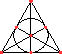
\includegraphics[width=0.6\linewidth]{Mathematics/2nd/Linear_geometry/Images/fano.tex} 
        \captionof{figure}{Fano configuration.}
        \label{fan}
    \end{minipage}
    \item It is the unique projective plane of order 2.\footnote{A finite projective plane of order $n$ is a  projective plane in which every line has $n+1$ points and every point lies in $n+1$ lines.}
    \item It is the projective plane $P_2(\mathbb{F}_2)$.
\end{itemize}
\end{definition}
\begin{theorem}
If $n\geq 2$, Fano configuration is a theorem in $P_n(k)$ if and only if $\text{char}\,k=2$.
\end{theorem}
\begin{definition}
\textit{Pappus configuration} is a configuration of 9 points and 9 lines defined in either of the following ways:
\begin{itemize}
    \item It is the configuration described in the figure \ref{pap}.\par
    \begin{minipage}{\linewidth}
        \centering
        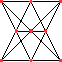
\includegraphics[width=0.6\linewidth]{Mathematics/2nd/Linear_geometry/Images/pappus.tex} 
        \captionof{figure}{Pappus configuration.}
        \label{pap}
    \end{minipage} 
    \item It is the configuration whose points are the elements of the group $\mathbb{Z}/9\mathbb{Z}$ and whose lines are triples $\{i,j,k\}$ such that $i+j+k=0$ where $i,j,k$ are different modulo 3.
    \item It is the configuration obtained from the affine plane over $\mathbb{F}_3$ eliminating three parallel lines.
\end{itemize}
\end{definition}
\begin{theorem}
Let $k$ be a division ring. Pappus configuration is a theorem in $P_n(k)$ if and only if $k$ is a field.
\end{theorem}
\subsubsection*{Desargues configuration}
\begin{definition}
Two triangles $ABC$ and $A'B'C'$ are said to be in \textit{perspective with respect to a point} if lines $AA'$, $BB'$ and $CC'$ intersect at the point $P$. This point is called \textit{centre of perspectivity}.
\end{definition}
\begin{definition}
Two triangles $ABC$ and $A'B'C'$ of sides $a,b,c$ and $a',b',c'$ respectively are said to be in \textit{perspective with respect to a line} if the points $a\cap a'$, $b\cap b'$ and $c\cap c'$ lie on the same line $r$. This line is called \textit{axis of perspectivity}.
\end{definition}
\begin{theorem}[Desargues' theorem]
If two triangles are in perspective with respect to a point, so are in perspective with respect to a line.\footnote{Desargues' theorem is valid in any axiomatic projective space of dimension 3 and, generally, in any axiomatic projective space that is a subvariety of an axiomatic projective space of dimension 3. In particular, it is valid in $P_n(k)$ for any division ring $k$ and $n\geq2$.}
\end{theorem}
\begin{definition}
\textit{Desargues configuration} is a configuration of 10 points and 10 lines defined in either of the following ways:
\begin{itemize}
    \item It is the configuration described in the figure \ref{des}.\par
    \begin{minipage}{\linewidth} 
        \centering
        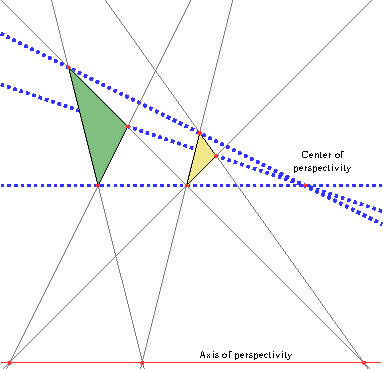
\includegraphics[width=0.75\linewidth]{Mathematics/2nd/Linear_geometry/Images/desargues.tex} 
        \captionof{figure}{Desargues configuration.}
        \label{des}
    \end{minipage}
    \item It is the configuration whose points are the elements of the set $S=\{1,2,3,4,5\}$ and whose lines are all subsets of cardinal 3 of $S$.
    \item It is the configuration created from two triangles that are simultaneously in perspective with respect to a point and in perspective with respect to a line. 
\end{itemize}
\end{definition}
\begin{definition}
Projective planes in which Desargues' theorem is not satisfied are called \textit{non-Desarguesian planes}.
\end{definition}
\begin{theorem}[Coordination theorem]
Let $X$ be an axiomatic projective space of finite dimension $n>1$ where Pappus' theorem is valid. Then there exist a field $k$ and an isomorphism $X\cong P_n(k)$.\footnote{If Pappus theorem is not valid but Desargues' theorem is, then $X\cong P_n(k)$ for some division ring $k$.}
\end{theorem}
\subsubsection*{Fundamental theorem of projective geometry and cross ratio}
\begin{theorem}[Fundamental theorem of projective geometry]
Let $f:\mathcal{P}(V)\rightarrow \mathcal{P}(W)$ be a collineation between projective spaces of finite dimension greater than $1$. Then, there exists an semilinear isomorphism $\phi:V\rightarrow W$ such that $f=P(\phi)$.
\end{theorem}
\begin{definition}[Cross ratio]
Let $A,B,C,D\in\mathcal{P}(V)$ be four collinear points lying on a line $L\in\mathcal{P}(V)$ with $A,B,C$ different. As we have $A=[v_1]$, $B=[v_2]$, $C=[v_3]$ and $D=[v_4]$ for some vectors $v_1,v_2,v_3,v_4\in V$ then $L=\langle v_1,v_2\rangle$. Therefore, $v_3=\lambda_1v_1+\lambda_2v_2$ and $v_4=\mu_1v_1+\mu_2v_2$, for some $\lambda_1,\lambda_2,\mu_1,\mu_2\in k$. We define the \textit{cross ratio between $A,B,C,D$} as $$(A,B,C,D):=\left\{\begin{array}{ccc}
    \displaystyle\frac{\lambda_2\mu_1}{\lambda_1\mu_2} & \text{si} & \lambda_1\mu_2\ne0, \\
    \infty & \text{si} & \lambda_1\mu_2=0.
\end{array}\right.$$ 
\end{definition}
\begin{definition}
Let $A,B,C,D\in\mathcal{P}(V)$ be four collinear points. If $(A,B,C,D)=-1$ we say the points $A,B,C,D$ form an \textit{harmonic ratio}.
\end{definition}
\begin{definition}
Let $a,b,c,d$ be four lines on a plane (with $a,b,c$ different) intersecting at the point $P$. Let $r$ be a different line such that $P\notin r$ and let $A:=a\cap r$, $B:=b\cap r$, $C:=c\cap r$, $D:=d\cap r$. We define the \textit{cross ratio between $a,b,c,d$} as $$(a,b,c,d):=(A,B,C,D).$$
\end{definition}
\begin{definition}
Let $X$ be a projective space such that $\dim X\geq 2$. Let $L_1,L_2\in X$ be two lines intersecting at the point $P\in X$ and $f:L_1\rightarrow L_2$ be a function such that $f(A)=L_2\cap PA$. We say $f$ is a \textit{prespectivity}. The composition of prespectivities is called a \textit{projectivity}.
\end{definition}
\begin{theorem}
If $f:L_1\rightarrow L_2$ is a projectivity, then $f$ preserves cross ratio, that is: $$(f(A),f(B),f(C),f(D))=(A,B,C,D).$$
\end{theorem}
\begin{theorem}
Let $V$ be a 2-dimensional vector space and $f:\mathcal{P}(V)\rightarrow \mathcal{P}(V)$ be a bijection. There exists linear map $\phi:V\rightarrow V$ such that $f=P(\phi)$ if and only if $f$ preserves cross ratio.
\end{theorem}
\subsubsection*{Plücker coordinates}
\begin{prop}
Let $r\in\mathcal{P}_3(k)$ be a line and $A,B\in r$ two points with coordinates $A=\{a_0,a_1,a_2,a_3\}$ and $B=\{b_0,b_1,b_2,b_3\}$. Consider the matrix: $$A=\begin{pmatrix}
a_0 & a_1 & a_2 & a_3 \\
b_0 & b_1 & b_2 & b_3 \\
\end{pmatrix}$$ Now consider the six minors of $A$:
\begin{gather*}
    p_{01}=\begin{vmatrix}
a_0 & a_1 \\
b_0 & b_1 \\
\end{vmatrix},\quad p_{02}=\begin{vmatrix}
a_0 & a_2 \\
b_0 & b_2 \\
\end{vmatrix},\quad p_{03}=\begin{vmatrix}
a_0 & a_3 \\
b_0 & b_3 \\
\end{vmatrix},\\ p_{23}=\begin{vmatrix}
a_2 & a_3 \\
b_2 & b_3 \\
\end{vmatrix},\quad p_{31}=\begin{vmatrix}
a_3 & a_1 \\
b_3 & b_1 \\
\end{vmatrix},\quad p_{12}=\begin{vmatrix}
a_1 & a_2 \\
b_1 & b_2 \\
\end{vmatrix}.
\end{gather*}
The coordinates $\{p_{01},p_{02},p_{03},p_{23},p_{31},p_{12}\}$ doesn't depend on the points $A,B$ on the line $r$. We define the \textit{Plücker coordinates of $r$} as the coordinates $\{p_{01},p_{02},p_{03},p_{23},p_{31},p_{12}\}$ 
\end{prop}
\begin{prop}
Two lines are equal if and only if have the same Plücker coordinates.
\end{prop}
\begin{prop}
Let $r$ be a line with Plücker coordinates $\{p_{01},p_{02},p_{03},p_{23},p_{31},p_{12}\}$. Then the points $x=\{x_0,x_1,x_2,x_3\}\in r$ satisfy $$\begin{pmatrix}
p_{12} & -p_{02} & p_{01} & 0 \\
-p_{31} & -p_{03} & 0 & p_{01} \\
p_{23} & 0 & -p_{03} & p_{02} \\
0 & p_{23} & p_{31} & p_{12} 
\end{pmatrix}\begin{pmatrix}
x_0\\
x_1\\
x_2\\
x_3
\end{pmatrix}=\begin{pmatrix}
0\\
0\\
0\\
0
\end{pmatrix}.$$
\end{prop}
\subsection{Affine geometry}
\subsubsection*{Affine space}
\begin{definition}
Let $V$ be a vector space over a field $k$. An \textit{affine space over $V$} is a set $\mathbb{A}$ together with a map:
\begin{align*}
    \mathbb{A}\times V&\rightarrow \mathbb{A}\\
    (P,\vec{v})&\mapsto P+\vec{v}
\end{align*}
such that:
\begin{enumerate}
    \item $P+\vec{0}=P$ for all $P\in X$.
    \item $P+(\vec{v}+\vec{w})=(P+\vec{v})+\vec{w}$ for all $P\in X$ and $\vec{v},\vec{w}\in V$.
    \item For all $P,Q\in X$ $\exists!\vec{v}\in V:Q=P+\vec{v}$. We denote the vector $\vec{v}$ by $\overrightarrow{PQ}$.
\end{enumerate}
\end{definition}
\begin{definition}
Let $\mathbb{A}$ be an affine space associated to a vector space $V$ over a field $k$.\footnote{From now on for simplicity we we will only refer to the affine space by mentioning the set $\mathbb{A}$ without mentioning the associated vector space $V$ over a field $k$.} We define the \textit{dimension of $\mathbb{A}$} as $\dim\mathbb{A}=\dim V$.
\end{definition}
\begin{prop}
Let $\mathbb{A}$ be an affine space, $P,Q,R,S\in\mathbb{A}$ and $u,v\in V$. Then, the following properties are satisfied:
\begin{enumerate}
    \item $\overrightarrow{PQ}=\overrightarrow{0}\iff P=Q$.
    \item $\overrightarrow{PQ}=-\overrightarrow{QP}$.
    \item $\overrightarrow{PQ}+\overrightarrow{QR}=\overrightarrow{PR}$.
    \item $\overrightarrow{PQ}=\overrightarrow{RS}\implies\overrightarrow{PR}=\overrightarrow{QS}$.
\end{enumerate}
\end{prop}
\begin{definition}
Let $\mathbb{A}$ be an affine space, $P_1,\ldots,P_n\in\mathbb{A}$ and $\lambda_1,\ldots,\lambda_n\in k$ such that $\lambda_1+\cdots+\lambda_n=1$. Given an arbitrary point $O\in\mathbb{A}$, we define the \textit{affine combination of $P_1,\ldots,P_n$} as $$\lambda_1P_1+\cdots+\lambda_nP_n:=O+\left(\lambda_1\overrightarrow{OP_1}+\cdots+\lambda_n\overrightarrow{OP_n}\right).$$ We say the points $P_1,\ldots,P_n$ are \textit{affinely independents} if the vectors $\overrightarrow{P_1P_2},\ldots,\overrightarrow{P_1P_n}$ are linearly independent.
\end{definition}
\begin{definition}
Let $\mathbb{A}$ be an affine space and $P_1,\ldots,P_r\in\mathbb{A}$. The \textit{barycenter of the points $P_1,\ldots,P_r$} is $$B:=\frac{1}{r}\left(P_1+\cdots+P_n\right).$$
\end{definition}
\subsubsection*{subvarieties and Gra\ss mann formula}
\begin{definition}
Let $\mathbb{A}$ be an affine space. If $P\in\mathbb{A}$ and $F$ is a vector subspace of $V$, then an \textit{affine subvariety of $\mathbb{A}$} is the set: $$P+F:=\{P+v\in\mathbb{A}:v\in F\}=\{Q\in\mathbb{A}:\overrightarrow{PQ}\in F\}.$$ We say $F$ is the \textit{director subspace of the subvariety $P+F$}. If $\dim F=m$, then $\dim (P+F)=m$. If $m=1$, we say the subvariety is \textit{line}. If $m=\dim\mathbb{A}-1$, we say la subvariety is a \textit{hyperplane}.
\end{definition}
\begin{prop}
Let $P+F$ be an affine subvariety of an affine space $\mathbb{A}$. Then if $Q\in P+F$, we have $P+F=Q+F$.
\end{prop}
\begin{definition}
Two subvarieties $P+F$ and $Q+G$ are said to be \textit{parallel} if $F\subseteq G$ or $G\subseteq F$.
\end{definition}
\begin{definition}
Let $Y,Z$ be two subvarieties of an affine space $\mathbb{A}$ such that $Y\cap Z\ne\emptyset$ and let $F,G$ be the director subspaces of $Y,Z$, respectively. Then if $P\in Y\cap Z$, we have that $Y\cap Z$ is a subvariety of $\mathbb{A}$ and $Y\cap Z=P+F\cap G$.
\end{definition}
\begin{definition}
Let $Y=P+F,Z=Q+G$ be two subvarieties of an affine space $\mathbb{A}$. We define its \textit{sum} as the subvariety $$Y+Z:=P+\left(F+G+\langle\overrightarrow{PQ}\rangle\right).\footnote{As expected, $Y+F$ is the smallest subvariety containing $Y\cup Z$.}$$ 
\end{definition}
\begin{theorem}[Affine Gra\ss mann formulas]
Let $L_1=P_1+F_1,L_2=P_2+F_2$ be two subvarieties of an affine space $\mathbb{A}$. Then:
\begin{itemize}
    \item If $L_1\cap L_2\ne\emptyset$, then $$\dim (L_1+L_2)=\dim L_1+\dim L_2-\dim (L_1\cap L_2).$$
    \item If $L_1\cap L_2=\emptyset$, then $$\dim (L_1+L_2)=\dim L_1+\dim L_2-\dim (F_1\cap F_2)+1.$$
\end{itemize}
\end{theorem}
\subsubsection*{Coordinates and equations}
\begin{definition}
An affine frame in an affine space $\mathbb{A}$ is a pair $\mathcal{R}=\{P;\mathcal{B}\}$ formed by a point $P\in\mathbb{A}$ and a basis $\mathcal{B}=(e_1,\ldots,e_n)$ of $V$. The point $P$ is called the \textit{origin} of this affine frame.
\end{definition}
\begin{definition}
Let $\mathcal{R}=\{P;\mathcal{B}\}$, $\mathcal{B}=(e_1,\ldots,e_n)$, be an affine frame in an affine space $\mathbb{A}$ and let $Q\in\mathbb{A}$. We define \textit{affine coordinates of $Q$} as $$Q=(\lambda_1,\ldots,\lambda_n)\iff\overrightarrow{PQ}=\lambda_1e_1+\cdots+\lambda_ne_n.$$
\end{definition}
\begin{prop}
Let $\mathbb{A}$ be an affine space and $P_0,\ldots,P_n\in\mathbb{A}$ be points satisfying the following equivalent properties:
\begin{enumerate}
    \item The points are affinely independent.
    \item There is no proper subvariety containing all of them.
    \item $P_0+\cdots+P_n=\mathbb{A}$.
    \item The vectors $\overrightarrow{P_0P_1},\ldots,\overrightarrow{P_0P_n}\in V$ are linearly independent.
\end{enumerate}
Then $\mathcal{R}=\{A_0;\overrightarrow{P_0P_1},\ldots,\overrightarrow{P_0P_n}\}$ is an affine frame in $\mathbb{A}$.
\end{prop}
\begin{definition}
Let $\{\lambda_0,\ldots,\lambda_n\}$ be homogeneous coordinates of a projective space $\mathcal{P}(V)$ and $(\mu_1,\ldots,\mu_n)$ affine coordinates of an affine space $\mathbb{A}$. We call \textit{homogenization} the transformation of affine coordinates to homogeneous coordinates as follows: $$(\mu_1,\ldots,\mu_n)\mapsto\{\mu_1,\ldots,\mu_n,1\}.$$ Similarly, we call \textit{deshomogenization} the transformation of homogeneous coordinates to affine coordinates as follows: $$\{\lambda_0,\ldots,\lambda_n\}\mapsto\left(\frac{\lambda_0}{\lambda_n},\ldots,\frac{\lambda_{n-1}}{\lambda_n}\right).$$
\end{definition}
\begin{definition}
Let $\mathcal{R}=\{P;\mathcal{B}\}$, $\mathcal{B}=(e_1,\ldots,e_n)$, be an affine frame in an affine space $\mathbb{A}$ and $L=Q+F$ a subvariety of $\mathbb{A}$. Let $Q=(q_1,\ldots,q_n)$ be a point and $(v_1,\ldots,v_r)$ a basis of $F$. We call \textit{parametric equations of $L$} the equations $$(x_1,\ldots,x_n)=(q_1,\ldots,q_n)+\sum_{i=1}^r\lambda_iv_i.$$ If $\lambda_1,\ldots,\lambda_r\in k$ we get the coordinates of $(x_1,\ldots,x_n)$. If $\displaystyle v_j=\sum_{i=1}^n\alpha_i^je_i$, $j=1,\ldots,r$ we can rearrange the parametric equations to get: $$\begin{pmatrix}
x_1-q_1 \\
\vdots \\
x_n-q_n \\
\end{pmatrix}=\begin{pmatrix}
\alpha_1^1 & \cdots & \alpha_1^r \\
\vdots & & \vdots \\
\alpha_n^1 & \cdots & \alpha_n^r \\
\end{pmatrix}\begin{pmatrix}
\lambda_1 \\
\vdots \\
\lambda_r \\
\end{pmatrix}.$$ The \textit{Cartesian equations of $L$} are those obtained by equating to zero the minors of size $(r+1)\times(r+1)$ of the augmented matrix $\left(\alpha_i^j\mid x_i-q_i\right)$.
\end{definition}
\subsubsection*{Affinities}
\begin{definition}
A map $f:\mathbb{A}_1\rightarrow\mathbb{A}_2$ between two affine space over vector spaces $V_1,V_2$ is an \textit{affinity} if there exists linear map $\phi:V_1\rightarrow V_2$ such that for all $P\in X$, $\overrightarrow{v}\in V_1$ $$f(P+\overrightarrow{v})=f(P)+\phi(\overrightarrow{v}).\footnote{If $\phi$ is a semilinear map, then we say $f$ is a \textit{semiafinity}.}$$ We call the \textit{differential of $f$}, denoted by $df$, the map $\phi$. 
\end{definition}
\begin{prop}
Let $f:\mathbb{A}_1\rightarrow\mathbb{A}_2$ and $g:\mathbb{A}_2\rightarrow\mathbb{A}_3$ be affinities. Then $g\circ f:\mathbb{A}_1\rightarrow\mathbb{A}_3$ is a affinity and $d(g\circ f)=dg\circ df$.
\end{prop}
\begin{prop}
Let $f:\mathbb{A}_1\rightarrow\mathbb{A}_2$ be an affinity and $P,Q\in\mathbb{A}_1$. Then $$df(\overrightarrow{PQ})=\overrightarrow{f(P)f(Q)}.$$
\end{prop}
\begin{prop}
Let $f,g:\mathbb{A}_1\rightarrow\mathbb{A}_2$ be affinities such that $f(P)=g(P)$ for some $P\in\mathbb{A}_1$ and $df=dg$. Then, $f=g$.
\end{prop}
\begin{prop}
Let $f:\mathbb{A}_1\rightarrow\mathbb{A}_2$ be an affinity and $\lambda_1,\ldots,\lambda_r$ such that $\lambda_1+\cdots+\lambda_r=1$. Then $$f(\lambda_1P_1+\cdots+\lambda_rP_r)=\lambda_1f(P_1)+\cdots+\lambda_rf(P_r).$$
\end{prop}
\begin{prop}
Let $f:\mathbb{A}_1\rightarrow\mathbb{A}_2$ be an affinity and $L=P+F$ be a subvariety of $\mathbb{A}$. Then $f(P+F)$ is a subvariety of $\mathbb{A}$ and $$f(P+F)=f(P)+df(F).$$
\end{prop}
\begin{prop}
Let $f:\mathbb{A}_1\rightarrow\mathbb{A}_2$ be an affinity and $\mathcal{R}_1=\{P_1;(e_1,\ldots,e_n)\}$, $\mathcal{R}_2=\{P_2;(v_1,\ldots,v_m)\}$ affine frames of $\mathbb{A}_1$, $\mathbb{A}_2$, respectively. If $x=(x_1,\ldots,x_n)\in\mathbb{A}_1$ and $y=(y_1,\ldots,y_n)\in\mathbb{A}_2$ then 
$$\begin{pmatrix}
y_1 \\
\vdots \\
y_m \\
\end{pmatrix}=\begin{pmatrix}
\rho_1 \\
\vdots \\
\rho_m \\
\end{pmatrix}+M\begin{pmatrix}
x_1 \\
\vdots \\
x_n \\
\end{pmatrix}$$
o, equivalently,
$$\begin{pmatrix}
y_1 \\
\vdots \\
y_m \\
1 \\
\end{pmatrix}=\left(\begin{array}{@{\,}ccc|c@{\,}}
    & & &\rho_1\\
    & M & & \vdots\\
    & & & \rho_m\\
    \hline
    0 & \cdots & 0 &  1
\end{array}\right)\begin{pmatrix}
x_1 \\
\vdots \\
x_n \\
1 \\
\end{pmatrix}=M_{\mathcal{R}_1,\mathcal{R}_2}(f)\begin{pmatrix}
x_1 \\
\vdots \\
x_n \\
1 \\
\end{pmatrix}$$ where $M$ is the matrix associated with $df$ and $(\rho_1,\ldots,\rho_m)$ are the coordinates of $\overrightarrow{P_2f(P_1)}$ in the basis $(v_1,\ldots,v_m)$. Here, $M_{\mathcal{R}_1,\mathcal{R}_2}(f)$ denote the matrix of $f$ with respect to affine frames $\mathcal{R}_1,\mathcal{R}_2$.
\end{prop}
\subsubsection*{Examples of affinities}
\begin{definition}
Two affinities $f,g:\mathbb{A}\rightarrow\mathbb{A}$ are \textit{similar} if there exist a bijective affinity $h:\mathbb{A}\rightarrow\mathbb{A}$ such that $h^{-1}fh=g$.
\end{definition}
\begin{prop}
Two affinities $f,g$ are similar if there exist affine frames $\mathcal{R},\mathcal{R}'$ such that $M_\mathcal{R}(f)=M_{\mathcal{R}'}(g)$.
\end{prop}
\begin{definition}
A punt $P\in\mathbb{A}$ is a \textit{fixed point of $f:\mathbb{A}\rightarrow\mathbb{A}$} if and only if $f(P)=P$.
\end{definition}
\begin{definition}
A linear subvariety $L=P+F\subset\mathbb{A}$ is \textit{invariant under an affinity $f:\mathbb{A}\rightarrow\mathbb{A}$} if and only if $f(L)\subset L$.
\end{definition}
\begin{prop}
A linear subvariety $L=P+F\subset\mathbb{A}$ is invariant under an affinity $f:\mathbb{A}\rightarrow\mathbb{A}$ if and only if
\begin{enumerate}
    \item $df(F)\subset F$.
    \item $\overrightarrow{Pf(P)}\in F$.
\end{enumerate} In particular, a line $r=P+\langle\overrightarrow{v}\rangle$ is invariant under $f$ if and only if
\begin{enumerate}
    \item $\overrightarrow{v}$ is an eigenvector of $df$.
    \item $\overrightarrow{Pf(P)}\in\langle\overrightarrow{v}\rangle$.
\end{enumerate}
\end{prop}
\begin{prop}
If the set of fixed points of an affinity $f$, $\text{Fix}(f)$, is non-empty, then $\text{Fix}(f)$ is a subvariety.
\end{prop}
\begin{definition}
Let $f$ be an affinity. We define the \textit{invariance level of $f$}, $\rho(f)$, as $$\rho(f)=\min\{\dim L:f(L)\subset L\subset\mathbb{A}\}\in[0,\ldots,\dim\mathbb{A}].$$  
\end{definition}
\begin{definition}[Translations]
Let $\mathbb{A}$ be an affine space and $\overrightarrow{v}\ne 0$. A \textit{translation} with translation vector $\overrightarrow{v}$ is an affinity $T_{\overrightarrow{v}}:\mathbb{A}\rightarrow\mathbb{A}$ defined by $T_{\overrightarrow{v}}=P+\overrightarrow{v}$.
\end{definition}
\begin{prop}[Properties of translations]
Let $T_{\overrightarrow{v}}$ be a translation. Then:
\begin{enumerate}
    \item $\text{Fix}(T_{\overrightarrow{v}})=\emptyset$.
    \item Invariant lines are those with director subspace $\langle\overrightarrow{v}\rangle$.
    \item If $\mathcal{R}=\{P;(\overrightarrow{v},\overrightarrow{v_2},\ldots,\overrightarrow{v_n})\}$ is an affine frame, then $$M_\mathcal{R}(T_{\overrightarrow{v}})=\left(\begin{array}{cccc|c}
        1 & 0 & \cdots & 0 & 1\\
        0 & \ddots & \ddots & \vdots  & 0\\
        \vdots & \ddots & 1 & 0 & \vdots\\
        0 & \cdots & 0 & 1 & 0\\
        \hline
        0 & \cdots & 0 & 0 &  1
    \end{array}\right).$$
    \item All translations are similar and $\rho(T_{\overrightarrow{v}})=1$.
\end{enumerate}
\end{prop}
\begin{definition}[Reflections]
Let $\mathbb{A}$ be an affine space and suppose $\text{char}(k)\ne 2$. Let $H=P+E$ be a hyperplane of $\mathbb{A}$ and let $\overrightarrow{v}\notin E$. The \textit{reflections of $\overrightarrow{v}$ with respect to $H$} is the unique affinity $f:\mathbb{A}\rightarrow\mathbb{A}$ such that $f(P)=P$ for all $P\in H$ and such that $df(\overrightarrow{v})=-\overrightarrow{v}$. Usually $H$ is called the \textit{mirror of the reflection} and $\overrightarrow{v}$ the \textit{root of the reflection}.
\end{definition}
\begin{prop}[Properties of reflections]
Let $f$ be a reflection with root $\overrightarrow{v}$ and mirror $H=P+E$. Then:
\begin{enumerate}
    \item $\text{Fix}(f)=H$.
    \item Invariant lines are those contained on $H$ and those with director subspace $\langle\overrightarrow{v}\rangle$.
    \item If $\mathcal{R}=\{P;(\overrightarrow{v_1},\ldots,\overrightarrow{v_{n-1}},\overrightarrow{v})\}$ is  an affine frame such that $P\in H$ and $\overrightarrow{v_1},\ldots,\overrightarrow{v_{n-1}}\in E$, then $$M_\mathcal{R}(f)=\left(\begin{array}{cccc|c}
    1 & 0 & \cdots & 0 & 0\\
    0 & \ddots & \ddots & \vdots & 0\\
    \vdots & \ddots & 1 & 0 & \vdots\\
     0&\cdots & 0 & -1 & 0\\
    \hline
    0 & \cdots & 0 & 0 &  1\\
    \end{array}\right)$$
    \item All reflections are similar and $\rho(f)=0$.
\end{enumerate}
\end{prop}
\begin{definition}[Projections]
Let $\mathbb{A}$ be an affine space and $H$ a hyperplane of $\mathbb{A}$ with director subspace $E$ and let $\overrightarrow{v}\notin E$. The \textit{projection over $H$ in the direction of $\overrightarrow{v}$} is the affinity $f:\mathbb{A}\rightarrow\mathbb{A}$ such that $f(P)=P$ for all $P\in H$ and such that $df(\overrightarrow{v})=0$.
\end{definition}
\begin{prop}[Properties of projections]
Let $f$ be a projection over $H=P+E$ in the direction of $\overrightarrow{v}$. Then:
\begin{enumerate}
    \item $\text{Fix}(f)=H$.
    \item Invariant lines are those contained on $H$.
    \item If $\mathcal{R}=\{P;(\overrightarrow{v_1},\ldots,\overrightarrow{v_{n-1}},\overrightarrow{v})\}$ is  an affine frame such that $P\in H$ and $\overrightarrow{v_1},\ldots,\overrightarrow{v_{n-1}}\in E$, then $$M_\mathcal{R}(f)=\left(\begin{array}{cccc|c}
    1 & 0 & \cdots & 0 & 0\\
    0 & \ddots & \ddots & \vdots & 0\\
    \vdots & \ddots & 1 & 0 & \vdots\\
     0&\cdots & 0 & 0 & 0\\
    \hline
    0 & \cdots & 0 & 0 &  1\\
    \end{array}\right)$$
    \item All projections are similar and $\rho(f)=0$.
\end{enumerate}
\end{prop}
\begin{definition}[Homotheties]
An \textit{homothety} is an affinity $f:\mathbb{A}\rightarrow\mathbb{A}$ such that $df=\lambda id$, $\lambda\ne0,1$. This $\lambda$ is called the \textit{similitude ratio of the homothety}.
\end{definition}
\begin{prop}[Properties of homotheties]
Let $f$ be an homothety of similitude ratio $\lambda$. Then:
\begin{enumerate}
    \item $f$ has a unique fixed.
    \item If $\mathcal{R}=\{P;\mathcal{B}\}$ is an affine frame with $P\in\text{Fix}(f)$ and $\mathcal{B}$ an arbitrary basis, then $$M_\mathcal{R}(f)=\left(\begin{array}{ccc|c}
     & & & 0\\
    & \lambda Id & & \vdots\\
    & & & 0\\
    \hline
    0 & \cdots & 0 &  1\\
    \end{array}\right)$$
    \item Two homotheties are similar if and only if they have the same similitude ratio. Moreover, $\rho(f)=0$.
\end{enumerate}
\end{prop}
\begin{prop}
Let $T_{\overrightarrow{w}}$ be a translation and $R$ a reflection with root $\overrightarrow{v}$ with respect to the hyperplane $H=P+E$. Let $f=T_{\overrightarrow{w}}\circ R$. We take an affine frame $\mathcal{R}=\{P;(\overrightarrow{v_1},\ldots,\overrightarrow{v_{n-1}},\overrightarrow{v})\}$ such that $\overrightarrow{v}_1,\ldots,\overrightarrow{v}_{n-1}\in E$. Then if $\overrightarrow{w}=(w_1,\ldots,w_n)$ in this frame we have,
    $$M_\mathcal{R}(f)=\left(\begin{array}{cccc|c}
    1 & 0 & \cdots & 0 & w_1\\
    0 & \ddots & \ddots & \vdots & w_2\\
    \vdots & \ddots & 1 & 0 & \vdots\\
    0 & \cdots & 0 & -1 & w_n\\
    \hline
    0 & \cdots & 0 & 0 &  1\\
    \end{array}\right)$$
    \begin{enumerate}
        \item If $\overrightarrow{w}\in\langle\overrightarrow{v}\rangle\implies w_1=\cdots =w_{n-1}=0$ and therefore $f$ is a reflection with mirror the hyperplane $2x_n=w_n$.
        \item If $\overrightarrow{w}\notin\langle\overrightarrow{v}\rangle$ we say $f$ is a \textit{glide reflection}. In that case, if $\overrightarrow{w}=w_n\overrightarrow{v}+\overrightarrow{e}$ with $\overrightarrow{e}\in E$ and we take $\mathcal{R}=(P+\frac{w_n}{2}\overrightarrow{v};(\overrightarrow{e},\overrightarrow{e_2}\ldots, \overrightarrow{e_{n-1}},\overrightarrow{v}))$ we have $$M_\mathcal{R}(f)=\left(\begin{array}{cccc|c}
    1 & 0 & \cdots & 0 & 1\\
    0 & \ddots & \ddots & \vdots  & 0\\
    \vdots & \ddots & 1 & 0 & \vdots\\
     0&\cdots & 0 & -1 & 0\\
    \hline
    0 & \cdots & 0 & 0 &  1\\
    \end{array}\right).$$ The invariance level of glide reflections is $\rho(f)=1$.
    \end{enumerate}
\end{prop}
\subsubsection*{Fundamental theorem of affine geometry}
\begin{definition}[Simple ratio]
Let $A,B,C\in\mathbb{A}$ be three different collinear points. The \textit{simple ratio of $A,B,C$} is the unique scalar $\lambda:=(A,B,C)\in k$ such that $$\overrightarrow{AB}=\lambda\overrightarrow{AC}.$$
\begin{theorem}[Fundamental theorem of affine geometry]
Let $f:\mathbb{A}\rightarrow\mathbb{A}$ be a collineation of an affine space of dimension $n\geq 2$ over the field $k$ with more than two elements. Then $f$ is a semiaffinity.
\end{theorem}
\begin{prop}
Two affinities $f,g:\mathbb{A}\rightarrow\mathbb{A}$ are similar if and only if
\begin{enumerate}
    \item $df$ and $dg$ are similar.
    \item $\rho(f)=\rho(g)$.
\end{enumerate}
\end{prop}
\begin{theorem}
Let $f:\mathbb{A}\rightarrow\mathbb{A}$ be an affinity and $P\in\mathbb{A}$ a point. Let $\overrightarrow{v}:=\overrightarrow{Pf(P)}$. Then $$\rho(f)=\min\{r:(df-id)^r(\overrightarrow{v})\in\text{Im}(df-id)^{r+1}\}.$$
\end{theorem}
\begin{corollary}
If $f$ is a affinity and 1 is not an eigenvector of $df$, then $\rho(f)=0$.
\end{corollary}
\end{definition}
\subsubsection*{Euclidean affine spaces}
\begin{definition}
An \textit{Euclidean affine space} is an affine space such that the associated vector space is an Euclidean vector space.\footnote{Remember definition \ref{espai_euclidia}.}
\end{definition}
\begin{definition}
Let $\mathbb{A}$ be an Euclidean affine space. We define the \textit{distance between two points $P,Q\in\mathbb{A}$} as $$d(A,B):=\|\overrightarrow{AB}\|.$$ We define the \textit{segment delimited by $A$ and $B$} as $$\{P\in\mathbb{A}:P=\lambda A+(1-\lambda)B,\lambda\in[0,1]\}.$$
\end{definition}
\begin{prop}
Let $\mathbb{A}$ be an Euclidean affine space. Then the following properties are satisfied:
\begin{enumerate}
    \item $d(A,C)\leq d(A,B)+d(B,C)\quad$ \textit{(Triangular inequality)}.
\end{enumerate}
If $ABC$ is a right triangle with right angle at $A$, then:
\begin{enumerate}
    \setcounter{enumi}{1}
    \item $d(B,C)^2=d(A,B)^2+d(A,C)^2\quad$ \textit{(Pythagorean theorem)}.
\end{enumerate}
\end{prop}
\begin{definition}
Two subvarieties $L_1=P_1+F_1,L_2=P_2+F_2$ of an Euclidean affine space $\mathbb{A}$ are \textit{orthogonal}, $L_1\perp L_2$, if $F_1\perp F_2$.\footnote{Remember definition \ref{perpendicular}.}
\end{definition}
\begin{definition}
Let $L_1=P_1+F_1,L_2=P_2+F_2$ be two subvarieties of an Euclidean affine space $\mathbb{A}$. We define the \textit{distance between two affine subvarieties} as $$d(L_1,L_2):=\inf\{d(A_1,A_2):A_1\in L_1, A_2\in L_2\}.$$
\end{definition}
\begin{theorem}
Let $L_1=P_1+F_1,L_2=P_2+F_2$ be two subvarieties of an Euclidean affine space $\mathbb{A}$. Let $\overrightarrow{u}=\overrightarrow{u}_1+\overrightarrow{u}_2\in F_1+F_2$ and $\overrightarrow{v}\in(F_1+F_2)^\perp$ such that $\overrightarrow{P_1P_2}=\overrightarrow{u}+\overrightarrow{v}$. Then we have $$d(L_1,L_2)=\|\overrightarrow{v}\|=d(P_1+\overrightarrow{u}_1,P_2-\overrightarrow{u}_2).$$
\end{theorem}
\subsubsection*{Euclidean motions}
\label{LG-euclidean_motion}
\begin{definition}
Let $\mathbb{A}$ be an Euclidean affine space. A map $f:\mathbb{A}\rightarrow\mathbb{A}$ is an \textit{Euclidean motions} if $$d(f(A),f(B))=d(A,B)\quad\text{for all } P,Q\in\mathbb{A}.$$
\end{definition}
\begin{prop}
Let $\mathbb{A}$ be an Euclidean affine space. $f:\mathbb{A}\rightarrow\mathbb{A}$ is an Euclidean motion if and only if $f$ is a affinity and $df$ is a isometry.\footnote{Remember definition \ref{isometry}. From this we deduce that if $A\in\mathcal{M}_n$ is the matrix associated with an isometry, then $AA^t=I_n$.}
\end{prop}
\begin{prop}[Examples of Euclidean motions]
\hfill
\begin{itemize}
    \item Any translation $T_{\overrightarrow{v}}$ is an Euclidean motion. Moreover, $T_{\overrightarrow{u}}\sim T_{\overrightarrow{v}}$ (as Euclidean motions) if and only if $\|\overrightarrow{u}\|=\|\overrightarrow{v}\|.$
    \item An homothety $f$ of similitude ratio $\lambda$ is an Euclidean motion if and only if $\lambda=-1$. Moreover, all homotheties are similar as Euclidean motions.
    \item A reflection $f$ of mirror $H=Q+E$ and root $\overrightarrow{v}$ is an Euclidean motion if and only if $\langle\overrightarrow{v}\rangle\perp E$. This reflections are called \textit{orthogonal reflections}. If $\overrightarrow{n}$ is a unit normal vector to the mirror, then the orthogonal reflection is given by $$f(P)=P-2\langle\overrightarrow{QP},\overrightarrow{n}\rangle\overrightarrow{n}.$$
    \item \textit{Glide orthogonal reflections} are Euclidean motions.
    \item A rotation on the affine plane is an Euclidean motion, whose differential is a rotation of an angle other than zero. This affinity has a unique fixed point and if we take this point for an affine frame, its matrix in this frame will be $$\begin{pmatrix}
    \cos\alpha & -\sin\alpha & 0\\
    \sin\alpha & \cos\alpha & 0\\
    0 & 0 & 1\\
    \end{pmatrix}.$$
\end{itemize}
\end{prop}
\subsubsection*{Classification of Euclidean motions}
\begin{theorem}[Classification of isometries]
\hfill
\begin{enumerate}
    \item Two isometries are similar if and only if they have the same characteristic polynomial.
    \item For any isometry, there exists an orthonormal basis in which the matrix associated with the isometry is of the form  $$\begin{pmatrix}
    I_r &&&&\\
    & -I_s &&&\\
    && R_1 &&\\
    &&& \ddots &\\
    &&&& R_t\\
    \end{pmatrix}$$ where $r,s,t\geq 0$, $I_m$ denote the identity matrix of size $m\times m$ and each $R_i$ is a rotation with matrix $$R_i=\begin{pmatrix}
    \cos\alpha_i & -\sin\alpha_i\\
    \sin\alpha_i & \cos\alpha_i\\
    \end{pmatrix}.$$ with $\alpha_i\ne0,\pi$ for $i=1,\ldots,t$.
\end{enumerate}
\end{theorem}
\begin{definition}
Let $P\in\mathbb{A}$ be a punt of an Euclidean affine space and $f:\mathbb{A}\rightarrow\mathbb{A}$ an Euclidean motion. Express $$\overrightarrow{Pf(P)}=\overrightarrow{u}+\overrightarrow{v}\quad\overrightarrow{u}\in\ker(df-I),\overrightarrow{v}\in\text{Im}(df-I).$$ Then $\overrightarrow{u}_f:=\overrightarrow{u}$ is the \textit{glide vector of $f$}.
\end{definition}
\begin{prop}
The glide vector $\overrightarrow{u}_f$ has the following properties:
\begin{itemize}
    \item $df(\overrightarrow{u}_f)=\overrightarrow{u}_f$.
    \item $\overrightarrow{u}_f$ does not depend on the point $P$.
    \item If $\overrightarrow{u}_f=0\implies\rho(f)=0$. Otherwise, $\rho(f)=1$.
\end{itemize}
\end{prop}
\begin{theorem}[Classification of Euclidean motions]
Two Euclidean motions $f,g:\mathbb{A}\rightarrow\mathbb{A}$ are similar (as Euclidean motions) if and only if $df\sim dg$ (as isometries) and $\|\overrightarrow{u}_f\|=\|\overrightarrow{u}_g\|$.
\end{theorem}
\subsection{Quadrics}
\subsubsection*{Quadrics}
\begin{definition}
Let $\mathbb{A}$ an affine space of dimension $n$ over a field $k$. A \textit{quadric in $\mathbb{A}$} is a polynomial of second degree with $n$ variables, $p(x_1,\ldots,x_n)$, and coefficients in the field $k$ modulo the equivalence relation $$p(x_1,\ldots,x_n)\sim\lambda p(x_1,\ldots,x_n)\quad\text{if }\lambda\in k,\lambda\ne0.$$ The \textit{points of the quadric} $p(x_1,\ldots,x_n)$ are $$\{(a_1,\ldots,a_n)\in\mathbb{A}:p(a_1,\ldots,a_n)=0\}.$$
\end{definition}
\begin{definition}
A \textit{conic} is a quadric in a 2-dimensional space.
\end{definition}
\begin{definition}
Two quadrics $p,q$ of an affine space $\mathbb{A}$ are \textit{equivalent} if there exists a bijective affinity $f:\mathbb{A}\rightarrow\mathbb{A}$ such that $f(p)=q$.
\end{definition}
\begin{definition}
Let $\mathcal{P}_n(k)$ be a projective space of dimension $n$ over a field $k$. A \textit{quadric in $\mathcal{P}_n(k)$} is a homogeneous polynomial of second degree with $n+1$ variables, $p(x_1,\ldots,x_{n+1})$, and coefficients in the field $k$ modulo the equivalence relation $$p(x_1,\ldots,x_{n+1})\sim\lambda p(x_1,\ldots,x_{n+1})\quad\text{si }\lambda\in k,\lambda\ne0.$$ The \textit{points of the quadric} $p(x_1,\ldots,x_{n+1})$ are $$\{(a_1,\ldots,a_{n+1})\in\mathcal{P}_n(k):p(a_1,\ldots,a_{n+1})=0\}.$$
\end{definition}
\begin{definition}
Two quadrics $p,q$ in $\mathcal{P}_n(k)$ are \textit{equivalent} if there exists a homography $f:\mathcal{P}_n(k)\rightarrow\mathcal{P}_n(k)$ such that $f(p)=q$.
\end{definition}
\begin{theorem}
There is a bijective correspondence between quadrics of $k^n$ and quadrics of $\mathcal{P}_n(k)$ not divisible by $x_{n+1}$. Thus, the points of the affine quadric are the points of the projective quadric that are in the affine space.\footnote{Nevertheless, observe that two equivalent projective quadrics as projective quadrics may not be equivalent as affine quadrics.}
\end{theorem}
\begin{prop}
Let $\mathbb{A}$ be an affine space and $\mathcal{P}_n(k)$ a projective space, both of dimension $n$ and over the field $k$. Let $p$ be a quadric. 
\begin{itemize}
    \item\textit{Homogenization}: If $p(x_1,\ldots,x_n)\in\mathbb{A}$, then $$p(x_1,\ldots,x_n)\mapsto x_{n+1}^2p\left(\frac{x_1}{x_{n+1}},\ldots,\frac{x_n}{x_{n+1}}\right)\in\mathcal{P}_n(k).$$
    \item\textit{Deshomogenization}: If $p(x_1,\ldots,x_{n+1})\in\mathcal{P}_n(k)$, then $$p(x_1,\ldots,x_{n+1})\mapsto p(x_1,\ldots,x_n,1)\in\mathbb{A}.$$
\end{itemize}
\end{prop}
\subsubsection*{Four point of view of quadrics}
\begin{definition}
We say a bilinear form is \textit{anisotropic} or\textit{elliptic} if the unique isotropic vector is the null vector.
\end{definition}
\begin{theorem}
There is, expect for equivalence, only one symmetric bilinear form of dimension 2 such that it is non-singular and non-elliptic. We call this bilinear form \textit{hyperbolic plane}.
\end{theorem}
\begin{definition}
Let $\varphi:V\times V\rightarrow k$ a symmetric bilinear form. We define the \textit{quadratic form associated with $\varphi$} as 
\begin{align*}
    q:V&\rightarrow k\\
    \overrightarrow{u}&\mapsto\varphi(\overrightarrow{u},\overrightarrow{u}).
\end{align*} This map, clearly satisfies:
\begin{enumerate}
    \item $q(\lambda\overrightarrow{u})=\lambda^2\overrightarrow{u}$.
    \item $\displaystyle\varphi(\overrightarrow{u},\overrightarrow{v})=\frac{1}{2}\left(q(\overrightarrow{u}+\overrightarrow{v})-q(\overrightarrow{u})-q(\overrightarrow{v})\right)$.
\end{enumerate}
\end{definition}
\begin{prop}
Two symmetric bilinear forms $\varphi_1,\varphi_2$ over $V$ are equivalent if there exists an isomorphism $\phi:V\rightarrow V$ such that $\varphi_1(\overrightarrow{u},\overrightarrow{v})=\varphi_2(\phi(\overrightarrow{u}),\phi(\overrightarrow{v}))$ for all $\overrightarrow{u},\overrightarrow{v}\in V$.\newline
Two quadratic forms $q_1,q_2$ over $V$ are equivalent if there exists an isomorphism $\phi:V\rightarrow V$ such that $q_1(\overrightarrow{u})=q_2(\phi(\overrightarrow{u}))$ for all $\overrightarrow{u}\in V$. 
\end{prop}
\begin{theorem}
Symmetric bilinear forms, quadratic forms, symmetric matrices and homogeneous polynomials of degree 2 are equivalents ways to study quadrics.
\end{theorem}
\begin{definition}
A quadric is \textit{non-degenerate} if la its associated quadratic form is non-singular.
\end{definition}
\subsubsection*{Classification of quadratic forms and qua\-drics}
\begin{definition}
A \textit{quadratic space} is a pair $(V,q)$ where $V$ is a vector space over a field $k$ and $q$ is a quadratic form.
\end{definition}
\begin{definition}
Let $E_1=(V_1,q_1)$ and $E_2=(V_2,q_2)$ be two quadratic spaces. An \textit{isometry between $E_1$ and $E_2$}, $E_1\cong E_2$, is an isomorphism $\phi:V_1\rightarrow V_2$ such that $q_1(\overrightarrow{v})=q_2(\phi(\overrightarrow{v}))$ for all $\overrightarrow{v}\in V$.
\end{definition}
\begin{definition}
Let $(V,q)$ be a quadratic space. $V$ is \textit{totally isotropic} if all its vectors are isotropic.
\end{definition}
\begin{definition}
Let $(V,q)$ be a quadratic space. We define the \textit{rank of $V$} as $$\rho(V):=\dim V-\dim\text{Rad}(V).\footnote{If $A$ is the associated matrix of $q$, we have $$\text{rank}\,A=\rho(V).$$}$$
\end{definition}
\begin{theorem}[Witt's theorem]
Let $(V_i,q_i)$, $i=1,2,3,4$, be a quadratic spaces and assume that $(V_1,q_1)\perp (V_2,q_2)\cong (V_3,q_3)\perp (V_4,q_4)$. If $E_1\cong E_2$, then $F_1\cong (V_i,q_i)$.
\end{theorem}
\begin{definition}
Let $(V,q)$ be a quadratic space. We define the \textit{index of $V$} as
$$\iota(V):=\max\{\dim F:F\subseteq V\text{ and $F$ is totally isotopic}\}.$$
\end{definition}
\begin{theorem}
Let $E\subseteq V$ a totally isotopic subspace of maximum dimension and $(\overrightarrow{e}_1,\ldots,\\\overrightarrow{e}_r)$ a basis of $E$ (therefore, $r=\iota(V)$). Then, there exist vectors $\overrightarrow{e}_1',\ldots,\overrightarrow{e}_r'\in V$ such that each $H_i:=\langle\overrightarrow{e}_i,\overrightarrow{e}_i'\rangle$ is an hyperbolic plane and $V=H_1\perp\cdots\perp H_r\perp F$, where $F$ is anisotropic.
\end{theorem}
\begin{prop}
Let $(V,q)$ be a quadratic space and $M$ the associated matrix of $q$. Then $\dim V$, $\rho(V)$, $\iota (V)$ and $\det M$ modulo squares\footnote{That is, if $(V_1,q_1),(V_1,q_1)$ are two quadratic spaces and $M_i$, $i=1,2$, are the associated matrices to $q_1,q_2$, respectively, we have $\det M_1=a^2\det M_2$, $a\in k$.} are invariant for isometries. 
\end{prop}
\begin{theorem}[Classification of quadratic forms in $\mathbb{C}$]
If $k=\mathbb{C}$, two quadratic forms are equivalent if and only if they have the same rank. All quadratic forms of rank $r$ are equivalent to $$x_1^2+\cdots+x_r^2.$$
\end{theorem}
\begin{theorem}[Classification of quadratic forms in $\mathbb{F}_q$]
If $k=\mathbb{F}_q$ with $q$ odd, all quadratic form
of rank $n$ are equivalent to either of these two diagonal forms: 
\begin{gather*}
    x_1^2+\cdots+ x_n^2,\\
    x_1^2+\cdots+ x_{n-1}^2+\nu x_n^2,
\end{gather*}
where $\nu$ in not a square. Moreover, two quadratic forms are equivalent if and only if they have the same rank and determinant (modulo squares).
\end{theorem}
\begin{theorem}[Classification of quadratic forms in $\mathbb{R}$]
If $k=\mathbb{R}$, all quadratic forms
of rang $r$ are equivalent to the diagonal form 
$$\pm x_1^2\pm\cdots\pm x_r^2.$$ If we denote by $r^+$ the number of positive signs and by $r^-$ the number of negative signs, then two quadratic forms are equivalents if and only if they have the same values $(r^+,r^-)$.
\end{theorem}
\begin{theorem}[Classification of projective qua\-drics in $\mathbb{C}$]
If $k=\mathbb{C}$, two projective quadrics are equivalents if and only if they have the same rank.
\end{theorem}
\begin{theorem}[Classification of projective qua\-drics in $\mathbb{F}_q$]
If $k=\mathbb{F}_q$, there are (except of equivalence) this projective quadrics in each rank $n$:
\begin{itemize}
    \item If $n$ is odd: $$\displaystyle x_1^2+\cdots+ x_n^2.$$
    \item If $n$ is even: \begin{gather*}
    x_1^2+\cdots+ x_n^2,\\
    x_1^2+\cdots+ x_{n-1}^2+\nu x_n^2,
\end{gather*}
where $\nu$ in not a square.
\end{itemize}
\end{theorem}
\begin{theorem}[Classification of projective qua\-drics in $\mathbb{R}$]
If $k=\mathbb{R}$, two projective quadrics are equivalents if they have the same rank and index.
\end{theorem}
\begin{theorem}[Classification of affine quadrics]
Let $q_1,q_2$ be two affine quadrics. $q_1\sim q_2$ if and only if:
\begin{enumerate}
    \item $q_1\sim q_2$ as projective quadrics, that is, in $P_n(k)$.
    \item $q_1^\infty\sim q_2^\infty$ as quadrics in $H\cong P_{n-1}(k)$.\footnote{Here $q_i^\infty$ are the quadrics $q_i$ restricted to the hyperplane \textit{at infinity} $H$, that is, by agreement, to the hyperplane $x_{n+1}=0$.}
\end{enumerate}
\end{theorem}
\end{multicols}
\end{document}